\subsection{Preissmann scheme}\label{subse:preissmann_scheme}




\begin{equation}\label{eq:approximated_function}
	f_p \approx \frac{1}{2} (\theta \cdot f_j^{i+1}+(1-\theta)f_j^i)+\frac{1}{2}(\theta\cdot f_{j+1}^{i+1}+(1-\theta)f_{j+1}^i)
\end{equation}
Where $\theta$ is a weighting parameter ranging between 0 and 1, j index of cross section and i index of time level. 

\begin{figure}[H]
\centering
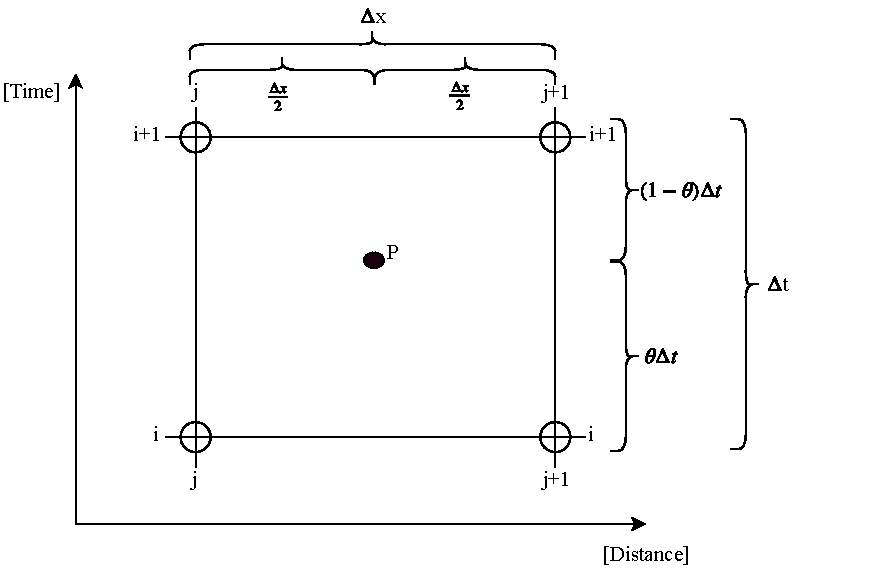
\includegraphics[width=.6\textwidth]{report/modeling/pictures/preissmann_scheme}
\caption{Preissmann grid scheme.}
\label{fig:preissmann_grid_scheme}%https://www3.epa.gov/npdes/pubs/bastre.pdf
\end{figure} 


\begin{equation}\label{eq:preissmann_time_derivatie}
	\frac{\partial f}{\partial t}\bigg \rvert_p \approx \frac{1}{2}\left(\frac{f_j^{i+1}-f_j^n}{\Delta t}+\frac{f_{j+1}^{i+1}-f_{j+1}^i}{\Delta t}\right)
\end{equation}

\begin{equation}\label{eq:preissmann_space_derivatie}
	\frac{\partial f}{\partial x}\bigg \rvert_p \approx (1-\theta)\frac{f_j^i-f_{j+1}^i}{\Delta x}+\theta \frac{f_j^{i+1}-f_{j+1}^{i+1}}{\Delta x}
\end{equation}

Applyed to the dynamuc equations 

\begin{equation}\label{eq:continuity_eq_preissmann}
	\theta \frac{Q_{j+1}^{i+1}-Q_j^{i+1}}{\Delta x}+(1-\theta)\frac{Q_{j+1}^i - Q_j^i}{\Delta x}+
	\frac{A_{j+1}^{i+1}-A_{j+1}^i}{\Delta t}+\frac{A_{j}^{i+1} - A_j^i}{\Delta t} = q(x,t)
\end{equation}
Where 
\begin{equation}
	q(x,t) = 0.25(q_j^i+q_j^{i+1}+q_{j+1}^{i+1}+q_j^{i+1})	
\end{equation}


Solved for Q(j+1,i+1)

\begin{equation}
	Q_{j+1}^{i+1} = - \frac{1}{2\theta}\left(A_{j+1}^{i+1}-H\right)\frac{\Delta x}{\Delta t}
\end{equation}
Where 
\begin{equation}
	H = \left(2(1-\theta)Q_j^i-2(1-\theta)Q_{j+1}^i+2\theta Q_j^{i+1}+2q(x,t)\Delta x\right)\frac{\Delta t}{\Delta x}- A_{j}^{i+1}+A_j^i+A_{j+1}^i
\end{equation}

\begin{equation}
		0=-Q_{j+1}^{i+1}  - \frac{1}{2\theta}\left(A_{j+1}^{i+1}-H\right)\frac{\Delta x}{\Delta t}
\end{equation}

\begin{equation}
		V=-Q_{j+1}^{i+1}  - \frac{1}{2\theta}\left(A_{j+1}^{i+1}-H\right)\frac{\Delta x}{\Delta t}
\end{equation}

\begin{equation}
	V = -Q_f\left(0,46-0,5cos\left(\pi \frac{h_{j+1}^{i+1}}{d}\right)+0,04cos\left(2\pi\frac{h_{j+1}^{i+1}}{d}\right)\right)\frac{\Delta t}{\Delta x}-\frac{1}{2\theta}\left(A_{j+1}^{i+1}-H\right)
\end{equation}

\begin{equation}
	V = -72\left(\frac{d}{4}\right)^{0.635}\pi\left(\frac{d}{2}\right)^2I_e^{0,5}\left(0,46-0,5cos\left(\pi \frac{h_{j+1}^{i+1}}{d}\right)+0,04cos\left(2\pi\frac{h_{j+1}^{i+1}}{d}\right)\right)\frac{\Delta t}{\Delta x}-\frac{1}{2\theta}\left(A_{j+1}^{i+1}-H\right)
\end{equation}

